%version of 02-27-19

\chapter{EXERCISES}
\label{ch:Exercises}


{\Arny
I think that solving specific examples of cubics via radicals, although specialized, does
involve useful skills for manipulating polynomials.  Therefore, I
propose to stop the general case here and leave a few exercises.  WHAT DO YOU THINK?}



{\Arny Because your geometric solution below involves just a single
  special quadratic --- and one that seems not to have other special
  interest --- I propose that we include it in some form of ENRICHMENT
  section.  }

{\ignore {\Denis It is interesting here to stress how hard it was to solve such equations. Algebra raised only in the second half of the last millenium.
However, there are several nice examples of geometrical solutions.
One of the oldest comes from babylonians in the 18th century BC.
The numeral system was in base 60, and the problem was to determine the length of the side of a square which was part of a larger rectangle.
The following figure details the process.}}
{\Denis Add here a small introduction about solving polynomial of degree 2 from El Kwharizmi, or remove it and put it as an exercice.}
\begin{figure}[htb]
\begin{center}
       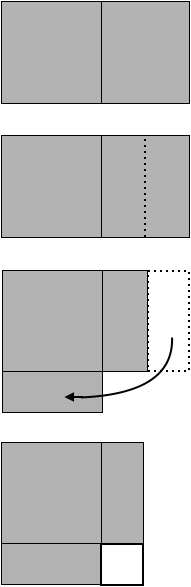
\includegraphics[scale=0.4]{FiguresArithmetic/tabletteMesopotamie}
\caption{Solving $x^2 + x = 45$.
The idea of the proof is to represent the left hand side by the square $x^2$ beside a rectangle $60 \times x$.
Then, split the right rectangle into two equal parts and move one part a the bottom of the left square.
The final figure shows the whole square whose surface is equal to $45$ plus the surface of the white square
whose surface is equal to $30 \times 30$.
In base $60$, this is $15$. 
$45+15 = 60$, thus, the big square is the unit square, its side is $60$.
Thus, the length of the initial square is equal to $60-30=30$.}
\label{fig:equationBabillon}
\end{center}
\end{figure}




\section{Summation}


\subsection{Compute $\Delta_n$ and sum of squares}

\ignore{$\Delta_n = \sum_{i=1}^{n} i = \frac{n(n+1)}{2}$

Use the same technique of writing the same sum by extracting the first and the last element provides a nice example.

We loose since the coefficient of the $\Delta_n$ is the same after these manipulations, but we can manage if we compute the \textit{next} sum, that is sum of the squares.
\medskip

$\Delta_{n+1} = 1 + \sum_{i=1}^{n+1} i $

$\Delta_{n+1} = (\sum_{i=1}^{n} i) + \frac{(n+1)(n+2)}{2}$
}

\subsection{Tetrahedral numbers}

The sum of the $\Delta_n$ is denoted by $\Theta_n$ and it is called a tetrahedral number:

$\Theta_n =  \sum_{k=1}^{n} \Delta_k$.

%We can show that: $\Theta_n = \frac{n.(n+1).(n+2)}{6}$

We proved the expression of $\Delta_n$ by mirroring the developed expression and adding term by term.
Similarly, a way to prove the expression of $\Theta_n$ is to consider three copies and organize them 
in order to obtain the expected result.
A tetrahedral number can be arranged as a triangle (see Figure~\ref{fig:TetrahedralBasic}).
\begin{figure}[h]
\begin{center}
        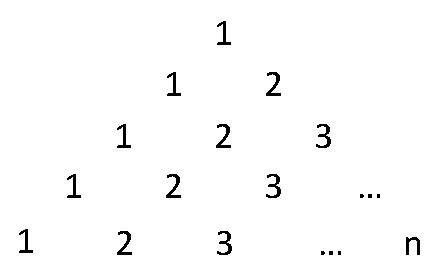
\includegraphics[scale=0.5]{FiguresArithmetic/TetrahedralBasic}
        \caption{Computing $\Theta_n$: basic triangle pattern.}
        \label{fig:TetrahedralBasic}
\end{center}
\end{figure}

The proof is obtained by Fubini's principle by rotating this triangle as shows in Figure~\ref{fig:Tetrahedral}.
\begin{figure}[h]
\begin{center}
        \includegraphics[scale=0.5]{FiguresArithmetic/Tetrahedral}
        \caption{Computing $\Theta_n$ using an adequate arrangement of $3$ triangles.}
        \label{fig:Tetrahedral}
\end{center}
\end{figure}

Sum up all the numbers in each row.

\begin{itemize}
\item 
The first row is equal to $n+2$.
\item
The second one is equal to $3 + 2(n-1)+3 = 2(n+2)$. 
\item
Let us sum up the elements in row $k$: 

$\Delta_k + k(n-k+1) + \Delta_k = k(k+1) +kn-k^2+k = k(n+2)$.
\end{itemize}

Conclusion:

The global sum is equal to $n+2$ times $(1+2+...+n)$.

Finally, $3 \Theta_n = (n+2) \Delta_n$.
\bigskip

Summary: we proved the following results:
\begin{itemize}
\item $Id_n = 1+1+ ... +1 = n$
\item $\Delta_n = 1+2+3+ ... +n = \frac{1}{2}.Id_n.(n+1)$
\item $\Theta_n = \Delta_1 + \Delta_2 + ... + \Delta_n = \frac{1}{3} .\Delta_n.(n+2)$
\end{itemize}

A natural question is if we can go further following the same pattern for computing 
$ \sum_{k=1}^{n} \Theta_k$, and so on.

Are you able to consider the challenge?


\section{More exercises}

\subsection{Graphical proofs 1}

Compute sum of squares with 3 copies and fill the 2D rectangle. 

The idea here is to consider $3$ copies of the sum of squares and to reorganize them in a more simple way 
(this is Fubini's principle).
The square of $a$ is represented as $a$ copies of the unit square.
The full process is depicted in figures Fig~\ref{fig:sumSquares1} to Fig~\ref{fig:sumSquares5}.

The height of the final rectangle is $\Delta_ n$ and its width is $2+2n-1=2n+1$. 

Thus, $3 \cdot S(n) = \Delta_n \cdot (2n+1)$, $S(n) = \frac{n(2n+1)(n+1)}{3}$.
\begin{figure}[ht]
\begin{center}
       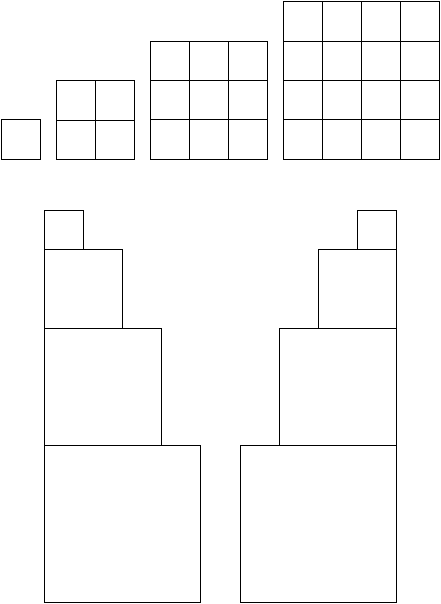
\includegraphics[scale=0.4]{FiguresMaths/SumSquares1}
\caption{Computing the sum of squares: initial configuration.}
       \label{fig:sumSquares1}
\end{center}
\end{figure}
\begin{figure}[ht]
\begin{center}
       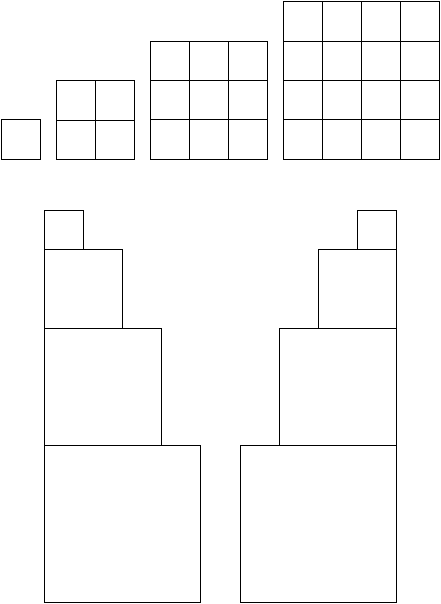
\includegraphics[scale=0.4]{FiguresMaths/SumSquares2}
\caption{Step 1 for computing the sum of squares: fill in the surface at the bottom.}
       \label{fig:sumSquares2}
\end{center}
\end{figure}
\begin{figure}[ht]
\begin{center}
       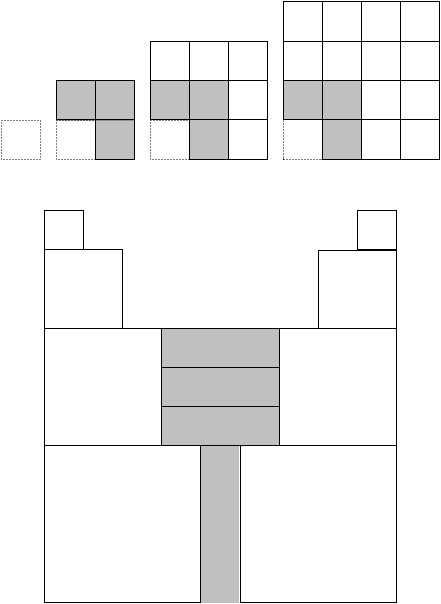
\includegraphics[scale=0.4]{FiguresMaths/SumSquares3}
\caption{Step 2 for computing the sum of squares.}
       \label{fig:sumSquares3}
\end{center}
\end{figure}
\begin{figure}[ht]
\begin{center}
       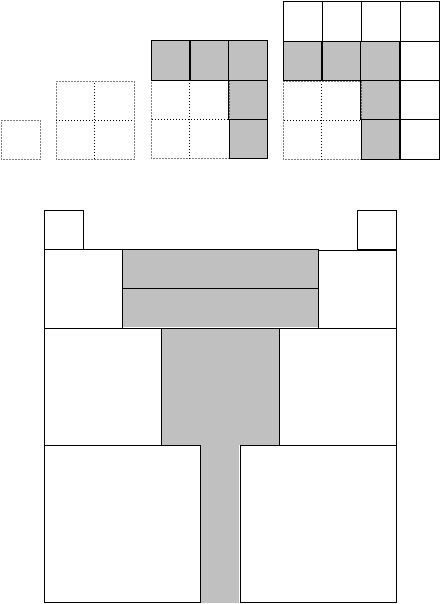
\includegraphics[scale=0.4]{FiguresMaths/SumSquares4}
\caption{Step 3 for computing the sum of squares.}
       \label{fig:sumSquares4}
\end{center}
\end{figure}
\begin{figure}[ht]
\begin{center}
       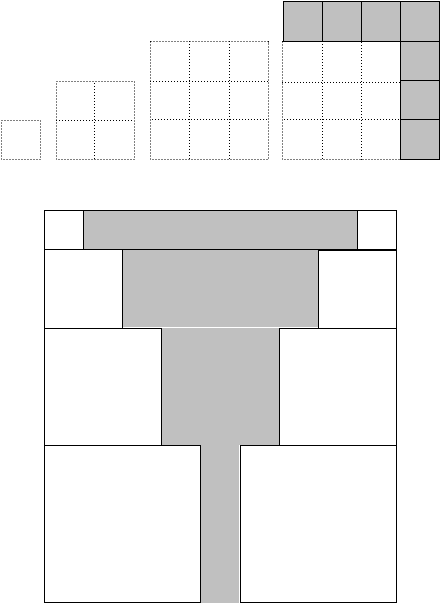
\includegraphics[scale=0.4]{FiguresMaths/SumSquares5}
\caption{Final step for computing the sum of squares: the rectangle is filled.}
       \label{fig:sumSquares5}
\end{center}
\end{figure}

\subsection{Graphical proofs 2}

Compute the sum of $(\frac{1}{4})^k = \frac{1}{3} $ using a graphical argument.
\bigskip

The solution is depicted in Fig.~\ref{Fig:SUmgeo1sur4}. 
\begin{figure}
\begin{center}
        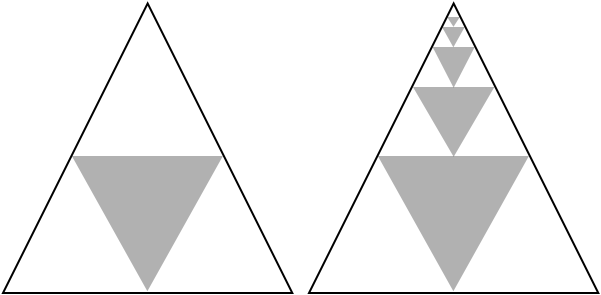
\includegraphics[scale=0.3]{FiguresArithmetic/SumGeometric1sur4}
        \caption{Graphical construction. Assuming the total area is 1, the area of the grey internal triangle (left) is $\frac{1}{4}$.
        As the grey area is one third at each layer (right), the whole area is $\frac{1}{3}$.
        By Fubini's principle, this area is the sum of the $\frac{1}{4^k}$ (for $k \geq 1$).}
        \label{Fig:SUmgeo1sur4}
\end{center}
\end{figure}

\subsection{Another proof for irrationality of $\sqrt{2}$}

Put the explicit question here.

The solution is depicted in Fig.~\ref{Fig:sqrtbisInit} and~\ref{Fig:sqrtbisFin} . 
\begin{figure}
\begin{center}
        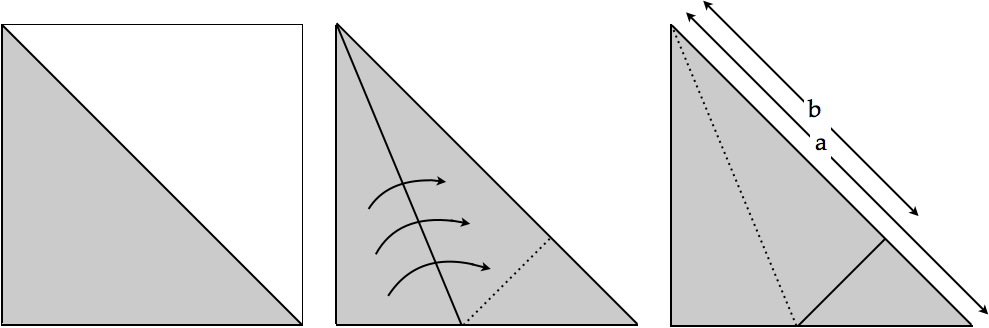
\includegraphics[scale=0.3]{FiguresArithmetic/sqrtbisInit}
        \caption{First step: folding the big triangle along the side.}
        \label{Fig:sqrtbisInit}
\end{center}
\end{figure}
\begin{figure}
\begin{center}
        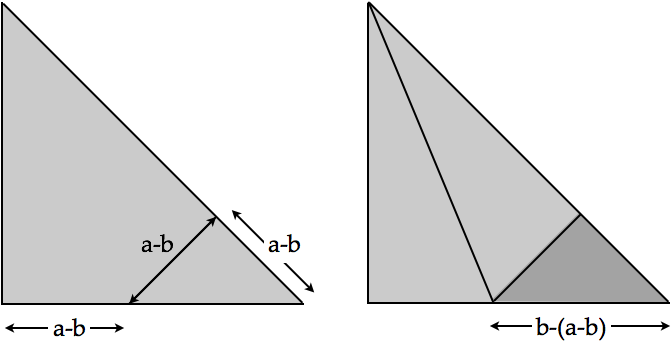
\includegraphics[scale=0.3]{FiguresArithmetic/sqrtbisFin}
        \caption{Second step. The sides of the small isocel triangle are integers.}
        \label{Fig:sqrtbisFin}
\end{center}
\end{figure}

\subsection{Harmonic series}

$H_{n} = \sum_{k=1}^{n} \frac{1}{k}$.

Another way to prove that the sum is infinite:
 
The analysis is as follows.
Group the terms according to powers of $2$. 
The sum within each group is between $\frac{1}{2}$ and $1$, thus,
$H_n > \frac{1}{2}.n$
\\

Another (more precise) way is to gather the terms 3 by 3 as follows:

$S_k = (\frac{1}{3k-1} + \frac{1}{3k} + \frac{1}{3k+1} )$ for $k\geq1$, 

$H = 1 + S_1 + ... + S_k + ... > 1 + 3.\frac{1}{3} + 3.\frac{1}{6} + ... + 3.\frac{1}{3k} + ... $

since $S_k > 3.\frac{1}{k} $.

The proof is by contradiction, if $H$ is finite, from the previous relation we have: $H > 1 + H$, which is obviously impossible.
\bigskip

Moreover, the first way of  bounding the sum tells us about its value (actually, we know the value at a factor of $2$):

$\frac{log(n)+1}{2} < H_n < log(n)+1$. Thus, $H_n = O(log(n))$

{\Denis Change the writing of O}



\section{Arithmetic}

\subsection{A fun result: complex
  multiplication via $3$ real multiplications}
\index{complex number!multiplication via 3 real multiplications}

\begin{prop}
%\label{thm:complex-mult-3real}
One can compute the product of two complex numbers using {\em three}
real multiplications rather than four.
\end{prop}

\begin{proof}
Although implementing (\ref{eq:complex-mult}) ``directly'' correctly
produces the product $\kappa = (a+bi) \cdot (c+di)$, there is another
implementation that is {\em more efficient}.  Specifically, the
following recipe computes $\kappa$ using only {\em three} real
multiplications instead of the four real multiplications of the
``direct'' implementation.  We begin to search for this recipe by
noting that our immediate goal is to compute both Re$(\kappa) = ac-bd$
and Im$(\kappa) = ad+bc$.  We can accomplish this by computing the
{\em three} real products
\begin{equation}
\label{eq:complex-mult-3a}
(a+b) \cdot (c+d); \ \ \ \ \
ac;  \ \ \ \ \ bd
\end{equation}
and then noting that
\begin{equation}
\label{eq:complex-mult-3b}
\begin{array}{lcl}
\mbox{Im}(\kappa) & = & (a+b) \cdot (c+d) - ac -bd, \\
\mbox{Re}(\kappa) & = & ac -bd
\end{array}
\end{equation}
We thereby achieve the result of the complex multiplication described
in (\ref{eq:complex-mult}) while using only {\em three} real
multiplications.

Of course, a full reckoning of the costs of the two implementations we
have discussed exposes the fact that the implementation that invokes
(\ref{eq:complex-mult-3a}) and (\ref{eq:complex-mult-3b}) uses {\em
  three} real additions rather than the {\em two} real additions of
the ``direct'' implementation.  But this entire exercise was
predicated on the observation that each real addition is much less
costly than a real multiplication, so trading one multiplication for
one addition is an unqualified ``win''.  \qed
\end{proof}

%%%%%%%%%%%%%%%%%%%%%%%%%%%%%%%%%%

\subsection{Karatsuba (Extension of the same method)} 


Notice that the previous technique is classical and it has been used in many other situations.
For instance while multiplying two integers in base 2.

Let us first recall the generic divide-and-conquer for designing algorithms.
\bigskip

\noindent \fbox{
\begin{minipage}{0.95\textwidth}
{\it Divide and conquer} is a paradigm for designing efficient algorithms for solving problems that can be
decomposed into sub-problems.

Let consider a problem of size $n$ that can be decomposed into $p$ sub-problems.
(notice, all sub-problems have the same size n/q).
\bigskip

\noindent {\bf Principle:}
\begin{enumerate}
\item Decompose the problem into $a$ sub-problems of size $\frac{n}{q}$.
\item Solve those sub-problems.
\item Reconstruct the solution of the initial problem.
\end{enumerate}

In general, the sub-problems are solved recursively (at least until a certain threshold).
The cost is governed by the following expression:

$T(n) = p.T(\frac{n}{q}) + c_1(n) + c_3(n)$ 

where $c_1(n)$ et $c_3(n)$ are the costs of phases (1) et (3).

Note: the resolution of this kind of equation is using the Master theorem of section~\ref{sec:linear-recurrence-general}.
\end{minipage}
}
\bigskip

Let $A=(a_na_{n-1}\ldots a_1)_2$ and $B=(b_nb_{n-1}\ldots b_1)_2$
be two long integers, and assume $n=2^k$ for some positive integer $k$.
The goal is to compute the product $A \times B$.

The standard (and naive) method is to compute the $n$ partial products 
$A=(a_na_{n-1}\ldots a_1)_2$ by each of the $b_i$, leading to $O(n^2)$ basic operations. 

The divide-and-conquer version of this problem is to break each integer into two parts
of $\frac{n}{2}$ bits each:

$A=(a_n\ldots a_{n/2+1})_2 2^{n/2}\ + (a_{n/2}\ldots a_1)_2$.

Denoting by $A_1$ and $A_2$ the two separate terms, we get:

$A.B = (A_1.B_1) 2^n + (A_1.B_2 + A_2.B_1) 2^{n/2} + A_2.B_2$
\bigskip

\textbf{Cost analysis} :
The previous computation requires 4 multiplications of integers of $n/2$ bits 
and 3 additions of integers with at most $2n$ bits. The multiplication of integers in base 2 by powers of 2 
correspond to simple shifts to the left. 

The cost is given by the following expression: $T(n) = 4.T(\frac{n}{2}) + f(n)$ where $f$ is a linear function
and $T(1) = 1$.

We obtain $T(n) = \Theta(n^2)$, same as for the naive algorithm.
\bigskip
 

The idea of Karatsuba is to decrease the number of multiplications 
(at the price of slightly increasing the additions/substractions) by using the following identity:

$A_1.B_1 + A_2.B_2 + (A_1-A_2).(B_2-B_1)$
\bigskip

We obtain:

$A.B = (A_1.B_1) 2^n + (A_1.B_1 + A_2.B_2 + (A_1-A_2).(B_2-B_1)) 2^{n/2} + A_2.B_2$


Cost analysis: 3 multiplications of $n/2$ bits

4 additions and 2 substractions of integers at most $2n$ bits. Again, using the Master Theorem leads to:

$T(n) = 3.T(\frac{n}{2}) + \theta (n) = n^{log_2 3}$


\subsection{A property about binomial coefficients}

Prove the following property by two ways (recurrence and by using a cominatorial argument
\begin{prop}
$\forall n,k$ $1 \leq k \leq n$

$k.{n choose k} = n.{{n-1} choose {k-1}}$
\end{prop}

\begin{proof}
to complete
\end{proof}



\subsection{Another fun result dealing with divisibility}

This exercice was a favorite question by Paul Erdos,
he often use this question to test the young students, apprentis mathematicians...
\bigskip

Let consider the $2n$ first integers.

Take any $n+1$ integers in this set and prove that there exists a pair $(p,q)$
such that $p$ divides $q$. 

The sketch of the proof is as follows.

\begin{enumerate}
\item
Let $\alpha_i$ be the elements of this set of cardinality $n+1$.

Write $\alpha_i = 2^k \times m$ where $m$ is odd (and $k \geq 0$).

Then, $m$ belongs to $\{1,3,5, \ldots, 2n-1 \}$
\item
From the pigeon hole principle, there are two numbers with the same value of $m$. 
\item 
Thus, $2^{k1} \times m$ and $2^{k2} \times m$.

$p$ is the smallest one, which divides $q$ (the largest one).
\end{enumerate}


\subsection{What's wrong?}

In this exercice, we investigate a proof which leads to a very surprising result...

\begin{enumerate}
\item
Let consider the infinite sum $A = 1-1+1-1+ \ldots$

and show that $A=\frac{1}{2}$ (hint: compute $1-A$)
\item
Let now consider the other infinite sum $B=2-3+4-5+6 \ldots$

and show that $B=\frac{1}{4}$ (hint: compute $A+B-1$)
\item 
Compute the sum of the integers $C=1+2+3+4+ \ldots$

and show that $C=-\frac{1}{12}$ (hint: compute $C-B=4+8+12+16+ \ldots$)
\end{enumerate}

What's wrong?

First, summing up positive number should be positive, 
and second, the sum of the integers should be infinite...




\subsection{A Fun Result: A ``Trick'' for Squaring Certain Integers}

Sometimes only basic knowledge is needed to craft amusing
``tricks''---we know that they are not really tricks at all!---that
are really rigorous applications of principles that we have learned.
Here is an ``old chestnut'' example that may inspire you to design
your own. 

If someone presents you with a number that has a numeral that ends in
$5$, then there is a simple way to square the number mentally.  For
instance, if someone says

\hspace{.25in}``$n = 25$''

\noindent
then you can instantly respond

\hspace{.25in}``$n^2 = 625$''

\noindent
If the challenge is

\hspace{.25in}``$n = 75$''

\noindent
then your response is

\hspace{.25in}``$n^2 = 5625$''

\noindent
Let's make this ``game'' mathematical.

\begin{prop}
\label{thm:75x65=4925}
Let $n$ be any number that has a $2$-digit decimal numeral of the form

\hspace{.25in}$\delta \ 5$ \ \ \ \ $(\delta \in \{ 0,1,2,3,4,5,6,7,8,9\})$.

\noindent
Then the square of $n$ is the integer

\hspace{.25in}$25 \ + \ \delta \cdot (\delta +1)$. 
\end{prop}

\begin{proof}
We can rewrite the premise of the proposition in the form
\[ n \ = \ 10 \cdot \delta + 5 \]
It is now easy to invoke Proposition~\ref{prop:(a+b)(c+d)} and the
distributive law to compute that

\[ n^2 \ = \ 100 \cdot \delta \cdot (\delta+1) + 25. \]
To wit: 
\[
\begin{array}{lclll}
n^2 & = & (10 \cdot \delta + 5)^2 & & \mbox{Given} \\
    & = & 100 \cdot \delta^2 \ + \ 100 \cdot delta \ + \ 25
              & & \mbox{the proposition} \\
    & = & 100 \cdot (\delta^2 \ + \ \delta) \ + \ 25
              & & \mbox{factoring: distributive law} \\
    & = & 100 \cdot \delta \cdot (\delta + 1) \ + \ 25
              & & \mbox{factoring: distributive law} \\
\end{array}
\]
A parlor trick has become a mathematical demonstration!
\qed
\end{proof}


\subsection{A fun result via geometric sums: When is integer  $n$
  divisible by $9$?}
\label{sec:divisible-by-9}

We now exploit our ability to evaluate geometric summations to
illustrate a somewhat surprising, nontrivial fact.  One can deduce
information about the divisibility of an integer $n$ from $n$'s
positional numerals.  We hope that this ``fun'' result will inspire
the reader to seek kindred numeral-encoded properties of numbers.

\begin{prop}
\label{thm:div-by-b-bar}
An integer $n$ is divisible by an integer $m$ if, and only if, $m$
divides the sum of the digits in the base-$(m+1)$ numeral for $n$.
\end{prop}

The most familiar instance of this result is phrased in terms of our
traditional use of base-$10$ (decimal) numerals. \\
{\it An integer $n$ is divisible by $9$ if, and only if, the sum of
  the digits of $n$'s base-$10$ numeral is divisible by $9$.}

\smallskip

\begin{proof}
({\it Argument for general number-base $b$}).
%
Of course, we lose no generality by focusing on numerals without
leading $0$'s, because leading $0$'s do not alter a numeral's sum of
digits.

Let us focus on the base-$b$ numeral for a number $n$ (so $b = m+1$ in
the statement of the proposition).  There therefore exist base-$b$
digits---i.e., integers from the set $\{0, 1, \ldots, b-1\}$---call
them $\delta_k \neq 0$, $\delta_{k-1}$, \ldots $\delta_1$, $\delta_0$,
such that
\[ n \ = \ \delta_k \cdot b^k + \delta_{k-1} \cdot b_{k-1} + \cdots +
\delta_1 \cdot b + \delta_0. \]
The sum of the digits of $n$'s base-$b$ numeral is, then
\[ s_b(n) \ \eqdef \ \delta_k + \delta_{k-1} + \cdots + \delta_1 +
\delta_0. \]
Let us calculate the difference $n - s_b(n)$ in the following manner,
digit by digit.
\begin{equation}
\label{eq:sum-of-digits}
\begin{array}{ccccccccccc}
n & = &
\delta_k \cdot b^k & + & \delta_{k-1} \cdot b^{k-1} & + & \cdots
  & + & \delta_1 \cdot b & + & \delta_0 \\
s_b(n) & = &
\delta_k & + & \delta_{k-1} & + & \cdots & + & \delta_1 & + & \delta_0 \\
\hline
n - s_b(n) & = &
\delta_k \cdot (b^k -1) & + &
\delta_{k-1} \cdot (b^{k-1} -1) & + &
\cdots & + &
\delta_1 \cdot (b-1) & & 
\end{array}
\end{equation}

\medskip

We now revisit summation (\ref{eq:geom-sum:b>1}).  Because $b$ is a
positive integer, so that $1 + b + \cdots + b^{a-2} + b^{a-1}$ is also
a positive integer, we infer that {\em the integer $b^a -1$ is
  divisible by $b-1$.}

We are almost home.  Look at the equation for $n - s_b(n)$ in the
system (\ref{eq:sum-of-digits}).  As we have just seen, every term on
the righthand side of that equation is divisible by $b-1$.  It follows
therefore, that the lefthand expression, $n - s_b(n)$, is also
divisible by $b-1$.
An easy calculation, which we leave to the reader, now shows that this
final fact means that $n$ is divisible by $b-1$ if, and only if,
$s_b(n)$ is.
\end{proof}



%%%%%%%%%%%%%%%%%%%%%%%%%%%%%%%%%%%%%

\section{Recurrences}



%%%%%%%%%%%%%%%%%%%%%%%%%%%%%%%%%%%

\section{Graphs}

\subsection{Spanning Trees}
\label{Appendix:spanningTrees}

Recall here the problem
\bigskip

There are mainly two ways for constructing such a MST, each one
emphasizes a different propriety of the MST, namely, avoid cycles and
minimize the span.  In both cases, the edges are sorted in increasing
order of weights.  More precisely, the first one constructs a subtree
which partially spans the graph by adding at each step the minimum
neighboring edge while the other add successively the edges of minimal
weights that do not create a cycle.

\subsection{Hamiltonian and Eulerian in de Bruijn}
\label{Appendix:hamiltonianDeBruijn}

\noindent {\bf (1)}
%
For any directed graph $\g$, the {\it line digraph} \index{line graph}
\index{line digraph} of $\g$, denoted $\Lambda(\g)$, is the following
directed graph.
\begin{itemize}
\item
The nodes of $\Lambda(\g)$ are the arcs of $\g$:
\[ \n_{{\Lambda}({\cal G})} \ = \ \a_{\fg} \]
\item
For each pair of arcs of $\g$ of the form
\[ \big[a_{x,y} = (x \ \rightarrow \ y) \big] \ \ \ \mbox{ and } \ \ \ 
\big[a_{y,z} = (y \ \rightarrow \ z) \big]
\]
i.e, arcs such that the endpoint of the first arc is the source of the
second arc, $\Lambda(\g)$ contains an arc $(a_{x,y} \ \rightarrow
\ a_{y,z})$.
\end{itemize}
The relevance of this topic to this section is that the line graph of
every de Bruijn network $\d_n$ is the ``next bigger'' de Bruijn
network, $\d_{n+1}$.  Let us verify this claim.

\begin{prop}
\label{thm:deBruin-linegraph}
For all $n \in \N^+$,
$\d_{n+1}$ is the line digraph of $\d_n$: $\d_{n+1} \ = \ \Lambda(\d_n)$.
\end{prop}

\begin{proof}
Each node of $\Lambda(\d_n)$ is an arc of $\d_n$, hence has the form
\[ (\beta x \ \rightarrow \ x \gamma) \]
for $x$ a length-$(n-1)$ binary string and $\beta, \gamma \in
\{0,1\}$.  Let us associate node $\beta x \gamma$ of $\d_{n+1}$ with
this node of $\Lambda(\d_n)$.

\smallskip

Note first that each arc of $\d_{n+1}$ has the form
\[ (\delta y \varepsilon \ \rightarrow \ y \varepsilon \varphi), \]
where $y$ is a length-$(n-2)$ binary string and $\delta, \varepsilon,
\varphi \in \{0,1\}$.  By our association of nodes of $\d_{n+1}$ with
arcs of $\d_n$, this arc of $\d_{n+1}$ does, indeed, correspond to two
successive arcs of $\d_n$.   The first of these successive arcs
{\em enters} node $y \varepsilon$ of $\d_n$; the second {\em leaves}
that node.

Note next that, given any two successive arcs of $\d_n$, say
\[
(\rho \sigma z \ \rightarrow \ \sigma z \tau) \ \ \ \mbox { and } \ \ \
(\sigma z \tau \ \rightarrow \  z \tau \xi)
\]
where $z$ is a length-$(n-2)$ binary string and $\rho, \sigma, \tau,
\xi \in \{0,1\}$, there is, indeed, an arc of $\d_{n+1}$ of the form
\[ (\rho \sigma z \tau \ \rightarrow \ \sigma z \tau \xi) \]
This means that the digraph $\d_{n+1}$ is identical to the digraph
$\Lambda(\d_n)$, modulo a renaming of nodes and arcs.\footnote{Technically,
  we are asserting that the digraphs ${\cal D}_{n+1}$ and ${\Lambda}({\cal D}_n)$ 
  are {\it isomorphic} to one another.  The topic of
  graph isomorphism is beyond the scope of this text, but our informal
  description provides all the details one would need to formalize the
  described isomorphism.}

The described correspondence between the nodes and arcs of $\d_{n+1}$
and $\Lambda(\d_n)$ completes the proof.  \qed
\end{proof}

\begin{figure}[hbt]
\begin{center}
       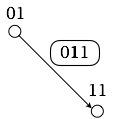
\includegraphics[scale=0.6]{FiguresGraph/dBlabelEdge}
\caption{Illustrating how to label each arc of a de Bruijn network by
  concatenating the labels of the nodes incident to the arc and
  compacting the common intermediate bits.  In the depicted example,
  the node-labels $01$ and $11$ combine to yield the arc-label $011$.}
  \label{fig:dBlabelEdge}
\end{center}
\end{figure}

\medskip

\noindent {\bf (2)}
{\it Eulerian cycles (or tours)}. \index{Eulerian cycle}
\index{Eulerian tour} A {\it directed Eulerian cycle} in a digraph
$\g$ is a directed cycle that contains each arc of $\g$ precisely
once.  We will see, later in this chapter, a truly elementary
argument, based on node-degrees, which proves that every de Bruijn
digraph has a directed Eulerian cycle.  This demonstration will
combine with Proposition~\ref{thm:deBruin-linegraph} to complete the
proof of Proposition~\ref{thm:deBruijn-Hamiltonian}.  \qed
%\end{proof}

\ignore{
\subsection{Coloring a planar graph with 5-colors}
\label{Appendix:5colors}

\begin{prop}[The $5$-Color Theorem for Planar Graphs \cite{Heawood90}]
\label{thm:P-5-colorability}
Every planar graph is $5$-colorable.
\end{prop}


\begin{proof}
The proof combines a sophisticated analysis of the structure of the
planar graph we wish to color with an induction that can be converted
into an efficient algorithm actually achieving the $5$-coloring.

\smallskip

For brevity, let us henceforth discuss only {\em valid} colorings,
i.e., colorings of a graph's nodes in which neighboring nodes get
different colors.

\smallskip

\noindent {\em Base of our induction.}
Because the $5$-clique $\k_5$ is obviously $5$-colorable, so also must
be all graphs having $\leq 5$ nodes.  Therefore, we know that any
non-$5$-colorable graph would have $\geq 6$ nodes.

\smallskip

\noindent {\em Inductive hypothesis.}
Assume, for induction, that every planar graph having $\leq n$ nodes
is $5$-colorable.

\smallskip

\noindent {\em Inductive extension.}
If the proposition were false, then there would exist a planar graph
$\g$ having $n+1$ nodes which is not $5$-colorable.  By
Lemma~\ref{thm:PlanarGraph-degree5}, $\g$ would have a node $v$ of
degree $\leq 5$.  The remainder of the proof focuses on the graph
$\g$, its minimal-degree node $v$, and on $v$'s $(d_v \leq 5)$
neighbors in $\g$.

Now, if there were a coloring of $\g$'s nodes in which $\leq 4$ colors
were used to color $v$'s neighbors, then the following analogue of the
coloring strategy of Proposition~\ref{thm:P-6-colorability} would
produce a $5$-coloring of $\g$.
\begin{enumerate}
\item
Remove node $v$ and its incident edges from $\g$, thereby producing
the $n$-node planar graph $\g'$.
\item
Produce a $5$-coloring of $\g'$ that uses only $4$ colors for the
nodes that are neighbors of $v$ in $\g$.
\item
($a$) Reattach node $v$ and its edges to $\g'$, thereby reconstituting
  $\g$.  ($b$) Color $v$ with whichever of the $5$ available colors is
  not used to color $v$'s neighbors.
\end{enumerate}

In order to proceed in pursuit of a contradiction, we must understand
what structural features of $\g$ make it impossible to use only $4$
colors on $v$'s neighbors when $5$-coloring $\g$.  There are three
important situations to recognize.
\begin{description}
\item[{\sf Case 1}.]
Node $v$ has degree $\leq 4$.

\smallskip

By definition, $\leq 4$ colors are used to color $v$'s neighbors in
this case.
\end{description}
Note that, in all remaining cases, node $v$ has precisely $5$
neighbors---or else, we would have invoked Case 1 to color $\g$ with
$5$ colors.
\begin{description}
\item[{\sf Case 2}.]
For some $5$-coloring of $\g$, $\geq 2$ neighbors of $v$ get the same
color.

\smallskip

Because $v$ has exactly $5$ neighbors, in this case, only $4$ colors
are used to color these neighbors.
\end{description}
In all remaining cases, the $5$ neighbors of $v$ receive distinct
colors.
\begin{description}
\item[{\sf Case 3}.]
For some $5$-coloring of $\g$, some two neighbors of $v$, call them
$v_1$ and $v_2$, reside in distinct components of $\g$ once $v$ and
its incident edges are removed from $\g$.

\smallskip

As before, let $\g'$ be the (in this case, disconnected) graph that
results when $v$ and its incident edges are removed from $\g$.  For $i
= 1,2$ Let $\g_i$ be the component of $\g'$ that contains node $v_i$.

Say that, under the $5$-coloring of $\g$ that we are focusing on,
$v_1$ is colored {\it red} and $v_2$ is colored {\it green}.

Let us recolor the nodes of $\g_1$ so that node $v_1$ is now colored
{\it green}.  (One needs only switch the colors {\it red} and {\it
  green} in the existing coloring of $\g_1$.)  It is always possible
to do this in a way that does not affect the valid coloring of $\g_2$
because $\g_1$ and $\g_2$ are mutually disjoint.

Once we have thus-recolored $\g_1$, we have a $5$-coloring of $\g$ for
which Case 2 holds.  (In fact, we can color node $v$ {\em red} when we
reattach it to $\g'$.)
\end{description}

\noindent
We now see that Cases 1--3 cannot prevent us from $5$-coloring $\g$, so
we are left with the following minimally constrained situation.
\begin{description}
\item[{\sf Case 4}.]
\begin{itemize}
\item
Every minimum-degree node of $\g$ has $5$ neighbors.

For the minimum-degree node $v$, let us call these neighbors $v_1$,
$v_2$, $v_3$, $v_4$, $v_5$, in clockwise order within the planar
drawing.
\item
In every $5$-coloring of $\g$, the neighbors of every minimum-degree
node receive distinct colors.

For node $v$, let us say that neighbor $v_i$ receives color $c_i$.
\end{itemize}
{\Denis Check carefully the ref to the figures...}

\begin{figure}[hbt]
\begin{center}
       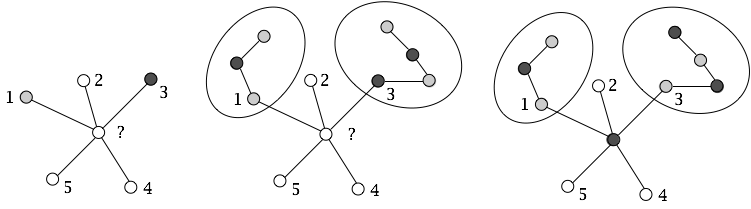
\includegraphics[scale=0.4]{FiguresGraph/5colorsCase1}
\caption{to be completed}
  \label{fig:5colorsCase1}
\end{center}
\end{figure}
The leftmost graph in Fig.~\ref{fig:5colorsCase1} depicts the portion of $\g$ comprising
node $v$ and its neighbors.  In the figure, we use integer $i$ to
denote, ambiguously, node $v_i$ and its assigned color $c_i$.  The
question mark ``?'' that ``colors'' node $v$ indicates that we do not
yet know what color to assign to $v$.  The other two graphs in the
figure depict schematically how we have dealt with Case 3 above.
{\Denis Clarify which are the concerned graphs here}
\begin{itemize}
\item
All neighbors of node $v$ remain in the same component of $\g$ when
$v$ and its incident edges are removed.
\end{itemize}
\end{description}
To analyze Case 4, we focus on nodes $v_1$ and $v_3$ in Fig.~\ref{fig:5colorsCase2}.
Importantly, these nodes have received distinct colors ($c_1$ and $c_3
\neq c_1$, respectively), and these nodes are not adjacent to one
another as one makes a clockwise sweep around node $v$.
\begin{figure}[hbt]
\begin{center}
       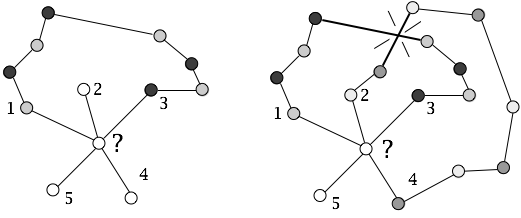
\includegraphics[scale=0.4]{FiguresGraph/5colorsCase2}
\caption{{\Denis to be completed}}
  \label{fig:5colorsCase2}
\end{center}
\end{figure}

Now take $\g$ and focus only on the nodes that are colored $c_1$ or
$c_3$ (as are $v_1$ and $v_3$, respectively) and on the nodes that are
colored $c_2$ or $c_4$ (as are $v_2$ and $v_4$, respectively).  One
sees from Fig.~\ref{fig:5colorsCase2} that:
\begin{itemize}
\item
$\g$ can, {\em but need not}, contain a path whose nodes alternate
  colors $c_1$ and $c_3$---call this a ``$c_1$-$c_3$ path'' between
  nodes $v_1$ and $v_3$.
\item
$\g$ can, {\em but need not}, contain a path whose nodes alternate
  colors $c_2$ and $c_4$---call this a ``$c_2$-$c_4$ path'' between
  nodes $v_2$ and $v_4$.
\item
$\g$ {\em cannot} contain both of the paths just described, i.e., a
  $c_1$-$c_3$ path between $v_1$ and $v_3$ {\em and} a $c_2$-$c_4$ path
  between $v_2$ and $v_4$.

{\em These two paths, if they existed, would cross one another---which
  is forbidden because $\g$ is a {\em planar} graph.}  See Figure 2.
\end{itemize}
It follows that {\em either} $\g$ does not contain a $c_1$-$c_3$ path
between $v_1$ and $v_3$ {\em or} $\g$ does not contain a $c_2$-$c_4$
path between $v_2$ and $v_4$.  Say, with no loss of generality, that
the former path does not exist.  Then we can switch colors $c_1$ and
$c_3$ beginning with node $v_1$ and obtain a coloring of $\g$ in which
$v_1$ and $v_3$ both receive the color $c_3$.  We can then proceed as
in Case 2 to get a $5$-coloring of $\g$.

This four-case analysis shows that we can always produce a
$5$-coloring of $\g$, which completes the proof.  \qed
\end{proof}
}
